\documentclass[10pt,twocolumn,letterpaper]{article}

\usepackage{cvpr}
\usepackage{times}
\usepackage{epsfig}
\usepackage{graphicx}
\usepackage{amsmath}
\usepackage{amssymb}
\usepackage{booktabs}
\usepackage{multirow}
\usepackage{float}
\usepackage{makecell}


% Include other packages here, before hyperref.

\usepackage[breaklinks=true,bookmarks=false]{hyperref}

\cvprfinalcopy % *** Uncomment this line for the final submission

\def\cvprPaperID{****}
\def\httilde{\mbox{\tt\raisebox{-.5ex}{\symbol{126}}}}

\setcounter{page}{1}
\begin{document}

%%%%%%%%% TITLE
\title{Physics-Constrained Thermal Map Prediction\\
for VLSI Chip Design}

\author{Fabian Molina\\
Stanford University\\
{\tt\small fmolina@stanford.edu}
\and
Ruben Carrazco\\
Stanford University\\
{\tt\small rubencarrazco@stanford.edu}
}

\maketitle

%%%%%%%%% ABSTRACT
\begin{abstract}
Predicting full-chip thermal distributions is a critical bottleneck in
VLSI design-space exploration: high-fidelity simulation is orders of
magnitude too slow for iterative floorplan optimization. Existing
data-driven surrogates achieve low in-distribution error but lack
physics grounding, leaving them susceptible to implausible predictions
under unseen die geometries or cooling conditions. We propose a
\emph{physics-constrained U-Net} that regresses dense steady-state
thermal heatmaps from a two-channel $256\times256$ floorplan and
power-density image, enforcing the 2D heat equation as a differentiable
Laplacian penalty with no simulator calls during training.

We train on 153 HotSpot-labeled layouts from the CircuitNet~2.0
GPU/accelerator benchmark and evaluate four model variants under
in-distribution and out-of-distribution (OOD) conditions spanning
unseen die thicknesses and convection resistances. Our best model
($\lambda{=}0.01$) achieves 0.895\,K RMSE and 0.841 hotspot IoU,
reducing in-distribution RMSE by 11\% over the MSE-only baseline. The
physics constraint provides modest convection-resistance OOD benefit
but does not improve die-thickness generalization, indicating that
stronger physics priors are needed for robust extrapolation.
\end{abstract}

%%%%%%%%% BODY TEXT
\section{Introduction}
Thermal management is a first-order constraint in modern VLSI design. On-chip hotspots cause performance throttling, increased leakage
current, and reduced mean time to failure. As process nodes continue
to shrink and power densities rise, accurate thermal prediction is
increasingly the binding constraint on achievable performance.
During design-space exploration, where automated placement and routing
tools evaluate candidate floorplans via simulated annealing, thermal
analysis must be repeated at every evaluation step. A single high-fidelity thermal
simulation using a tool like HotSpot~\cite{HotSpot} or ANSYS MAPDL
can take seconds to minutes per design; at $10^5$ evaluations per
optimization run, this cost is prohibitive.

Neural thermal surrogates address this bottleneck by learning to
approximate the simulator's output from cheap layout representations.
The input to our algorithm is a 2-channel $256\times256$ image: channel
1 encodes the post-placement floorplan (cell density), and channel 2
encodes the normalized power-density map derived from post-synthesis
switching activity. We use a convolutional neural network to output a
predicted $256\times256$ steady-state thermal heatmap in Kelvin. This
image-to-image regression formulation preserves the full spatial
structure of the temperature field, enabling precise localization of
hotspots, the regions that most directly drive thermal violations.

The core challenge is \emph{generalization}: a surrogate trained on a
finite set of chip configurations must remain reliable when deployed on
designs with different die geometries or cooling conditions than those
seen during training. In practice, VLSI designers routinely explore
package variants spanning a range of die thicknesses, substrate
materials, and heat-sink configurations; any deployed surrogate will
encounter parameter settings outside its training sweep. A model that
violates the heat equation under such shifts can actively mislead the
optimizer, steering candidate designs toward layouts that appear
thermally safe but fail sign-off simulation. Prior data-driven
surrogates achieve low in-distribution error but can produce physically
implausible extrapolations when parameters shift outside the training
regime, because nothing in their training objective prevents the model
from violating the underlying heat equation.

\textbf{This work combines image-based prediction with physics-informed
training.} We frame thermal prediction as image-to-image
regression, preserving the representational advantages of
convolutional architectures~\cite{UNet}, while augmenting the
training loss with a differentiable residual of the 2D steady-state
heat equation. The physics penalty is computed via a fixed $3\times3$
Laplacian convolution on the model's output, requiring no simulator
calls during training. Because the constraint penalizes predictions
that violate the heat equation regardless of the ground-truth label,
it acts as a physics-grounded regularizer that we hypothesized would
reduce OOD degradation on unseen die parameters.

Our main contributions are:
\begin{itemize}
  \item A \textbf{physics-constrained U-Net} with pixel-shuffle
    upsampling trained with a composite loss balancing MSE data
    fidelity and a heat equation residual penalty.
  \item An \textbf{OOD generalization study} evaluating models on
    die thickness and convection resistance values outside the
    training sweep, isolating the effect of the physics constraint.
  \item A \textbf{systematic ablation} over physics loss weighting
    $\lambda_\text{phys} \in \{0, 0.01, 0.1, 1.0\}$, showing that
    $\lambda{=}0.01$ achieves the best in-distribution performance
    and modest convection-resistance OOD benefit.
\end{itemize}

Our results show that the physics penalty primarily acts as an
in-distribution regularizer: the optimal $\lambda{=}0.01$ reduces
RMSE by 11\% over the MSE-only baseline and improves hotspot IoU by
2.7 percentage points. OOD behavior is asymmetric: the physics
constraint yields 8--11\% RMSE reduction under moderate
convection-resistance shifts but provides no benefit for
die-thickness generalization, where all U-Net variants degrade
similarly. These findings suggest that lightweight Laplacian
regularization is a practical tool for improving in-distribution
accuracy of neural thermal surrogates, but that stronger physics
priors or geometry-aware formulations are needed for robust
extrapolation across die parameters.

%------------------------------------------------------------------------
\section{Related Work}

\paragraph{Thermal simulation tools.}
HotSpot~\cite{HotSpot} is an open-source block-level RC-network
thermal simulator widely used in computer architecture research. Its
grid mode produces dense 2D steady-state heatmaps, making it directly
compatible with image-to-image framing and the natural choice for
ground-truth label generation at training scale. PACT~\cite{PACT}
is a higher-fidelity coupled electro-thermal simulator that captures
transient phenomena HotSpot cannot; however, its per-design runtime
makes it impractical for generating the hundreds of labeled layouts
required to train a surrogate. Both tools are simulation engines, not
surrogates: neither is designed for the fast, differentiable inference
required during design-space optimization.

\paragraph{Data-driven thermal surrogates.}
CircuitNet~2.0~\cite{CircuitNet2} is a large-scale benchmark dataset
for machine learning in chip design, providing post-placement
floorplans, power maps, and multiple analysis targets including
thermal. We use its GPU and AI accelerator designs as layout inputs,
generating our own HotSpot labels to control the die-parameter sweep.
DeepOHeat~\cite{DeepOHeat} applies operator learning to thermal
simulation and represents the current state-of-the-art on
in-distribution accuracy; it neither incorporates physics constraints
nor evaluates OOD generalization, leaving open whether predictions
remain physically consistent under distribution shift. Prior
encoder-decoder approaches~\cite{EncoderDecoderThermal} demonstrate
the viability of dense regression for thermal prediction but share
the same lack of physics grounding. ML-PACT~\cite{MLPACT} targets
transient thermal analysis and is not directly comparable to our
steady-state formulation.

\paragraph{Image-to-image translation.}
The pix2pix framework~\cite{pix2pix} established conditional GANs for
dense image prediction from spatial inputs. While powerful, adversarial
training is sensitive to hyperparameters, prone to mode collapse, and
provides no physical interpretability. Our formulation replaces the
adversarial objective with a physics-grounded loss, yielding stable
training and predictions that are explicitly penalized for violating
the heat equation.

\paragraph{U-Net and skip connections.}
U-Net~\cite{UNet} introduced encoder-decoder networks with lateral
skip connections for dense prediction in biomedical segmentation. Skip
connections concatenate high-resolution encoder features to the
corresponding decoder stage, preserving fine spatial detail: a
critical strength for hotspot localization, where the temperature
extremes rather than global structure drive design decisions. We adopt
the U-Net backbone with pixel-shuffle upsampling~\cite{PixelShuffle}
in place of bilinear or transposed convolution to reduce checkerboard
artifacts in the predicted thermal map.

\paragraph{Physics-informed learning.}
Raissi \etal~\cite{Raissi2019} introduced PINNs, embedding PDE
residuals as loss terms over collocation points to learn solutions to
forward and inverse problems. PINNs operate on point-wise coordinate
inputs and require retraining per problem instance, making them poorly
suited to the image-regression setting where a single forward pass must
generalize across many distinct layouts. We adapt the residual idea to
operate on the pixel grid of a convolutional output via a fixed
Laplacian filter, which is fully parallelizable over spatial dimensions,
compatible with mini-batch training on image data, and requires no
per-layout retraining, directly addressing the key limitation of
coordinate-based PINN formulations.

%------------------------------------------------------------------------
\section{Data}

\paragraph{Source.}
We use CircuitNet~2.0~\cite{CircuitNet2} as our source of chip
layout inputs. From the full dataset we select the GPU and AI
accelerator designs: Vortex-small (96 instances), Vortex-large (61
instances), and NVDLA-large (32 instances), for 189 instances total.
Each sample consists of a two-channel $256\times256$ image: channel~1
is the post-placement floorplan (macro-region feature) encoding block
boundaries and functional unit types; channel~2 is the power-density
map derived from post-synthesis switching activity estimates.
Figure~\ref{fig:data} shows a representative sample.

\paragraph{Label generation.}
We run HotSpot~\cite{HotSpot} in grid mode ($256\times256$ output)
on each layout using a multi-block $16\times16$ floorplan
decomposition. The training configuration uses a die thickness of
$150\,\mu\text{m}$ and a convective resistance of
$r_\text{convec}{=}0.1\,\text{K/W}$. Power-density values are
capped at $10\,\text{W}$ per tile to suppress outliers from unit
conversion. Label generation is parallelized across all 189 instances
using cloud-based serverless workers (Modal). For the OOD evaluation,
we re-run HotSpot at four additional thicknesses ($75$, $100$, $200$,
$300\,\mu\text{m}$) and four additional convective resistances
($r_\text{convec}\in\{0.01,\,0.05,\,0.20,\,0.50\}\,\text{K/W}$),
producing $189\times 8 = 1{,}512$ additional OOD labels. Thermal
labels are normalized per chip family using the training-split mean
and standard deviation, so each family's thermal range is mapped to a
consistent scale regardless of absolute power level.

\paragraph{Splits.}
We split instances randomly (seed~42) into 80/10/10 train/val/test
partitions within each family, yielding 153 training, 18 validation,
and 18 test instances. All three families appear in each partition.
The OOD evaluation uses the combined val and test sets
($18+18=36$ instances) re-evaluated under held-out physical parameters
(thickness and convective resistance) never seen during training.

\paragraph{Augmentation.}
We apply random horizontal and vertical flips during training.
Rotation is excluded because our discrete Laplacian kernel is
not rotation-equivariant and rotating a layout would invalidate
the physics constraint.

\begin{figure}[t]
\begin{center}
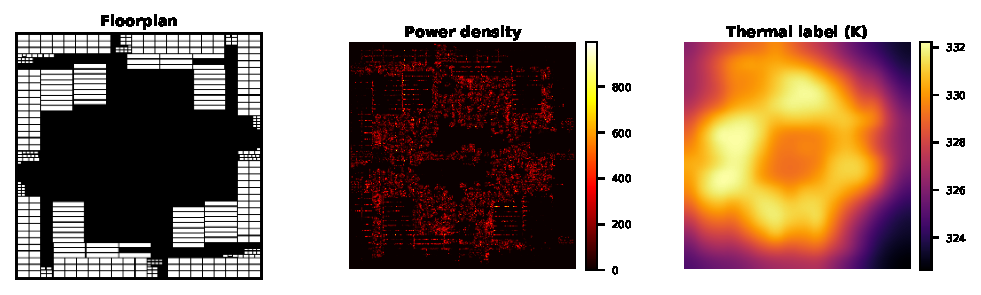
\includegraphics[width=\linewidth]{figures/data_figure}
\end{center}
\caption{Representative sample from the Vortex-large family.
\textbf{Left:} post-placement floorplan (macro-region feature);
dark regions are active logic blocks.
\textbf{Center:} power-density map derived from post-synthesis
switching activity; bright spots indicate high-power functional units.
\textbf{Right:} HotSpot steady-state thermal label (Kelvin);
the hotspot ring corresponds to the high-power region in the
power map. The model takes the floorplan and power map as a
2-channel input and predicts the thermal label.}
\label{fig:data}
\end{figure}

%------------------------------------------------------------------------
\section{Methods}

\subsection{Architecture}

Our primary model is a U-Net~\cite{UNet} with pixel-shuffle upsampling,
illustrated in Figure~\ref{fig:arch}. The encoder progressively
halves spatial resolution while doubling feature channels through
four stages; the decoder restores resolution using skip connections
from the corresponding encoder stages. The architecture is parameterized by base channel count $b$; we train with
$b {=} 32$ (${\approx}2$M parameters). The encoder progression is
$2 \to b \to 2b \to 4b \to 8b$, the bottleneck has $16b$ channels, and
the decoder mirrors this symmetrically back to a single output channel.
For $b {=} 32$: encoder goes $2 \to 32 \to 64 \to 128 \to 256$, bottleneck
has 512 channels.

\textbf{DoubleConv block.} Each encoder and decoder stage applies
two sequential $3\times3$ convolutions, each followed by batch
normalization and ReLU activation. The dilation parameter is
exposed for experimentation but defaults to 1. Padding equals
dilation, preserving spatial dimensions through each block.

\textbf{PixelShuffleUp block.} We upsample via a $1\times1$
convolution that expands the channel dimension by a factor of 4,
followed by a PixelShuffle~\cite{PixelShuffle} operation with
upscale factor 2:
\begin{equation}
  \text{PixelShuffleUp}(\mathbf{F}) =
  \text{PixelShuffle}_2\bigl(\text{Conv}_{1\times1}(\mathbf{F},\;
  C \to 4C')\bigr).
\end{equation}
This produces a $2\times$ spatially upsampled feature map with $C'$
channels. We prefer this over bilinear upsampling (sharper thermal
gradients) and transposed convolution (fewer checkerboard artifacts),
both of which matter for hotspot localization precision.

After upsampling, the decoder concatenates the skip-connected encoder
feature map and applies a DoubleConv block to fuse the two
resolutions. The output layer is a $1\times1$ convolution with no
activation function (linear regression for unbounded temperature values).

\textbf{Bottleneck regularization.} A spatial dropout layer
(\texttt{Dropout2d}, $p {=} 0.3$) is applied to the bottleneck output before
upsampling begins. This pushes the decoder to rely on skip-connected
encoder features rather than only the bottleneck representation.

\begin{figure*}[t]
\begin{center}
\begin{minipage}[t]{0.28\linewidth}
  \centering
  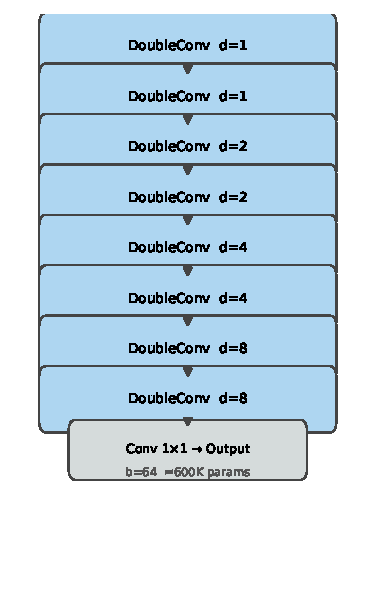
\includegraphics[width=\linewidth]{arch_plaincnn}\\[3pt]
  \small\textbf{(a) PlainCNN}\\[1pt]
  \small Eight DoubleConv blocks at full resolution with dilations
  $[1,1,2,2,4,4,8,8]$; no downsampling ($b{=}64$, ${\approx}600$K params).
\end{minipage}
\hfill
\begin{minipage}[t]{0.34\linewidth}
  \centering
  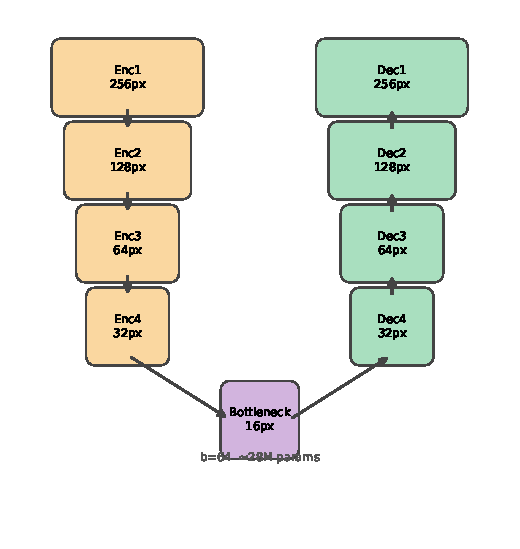
\includegraphics[width=\linewidth]{arch_encoderdecoder}\\[3pt]
  \small\textbf{(b) EncoderDecoder}\\[1pt]
  \small Four-stage encoder (MaxPool2d) and symmetric PixelShuffleUp
  decoder; no skip connections ($b{=}64$, ${\approx}28$M params).
\end{minipage}
\hfill
\begin{minipage}[t]{0.34\linewidth}
  \centering
  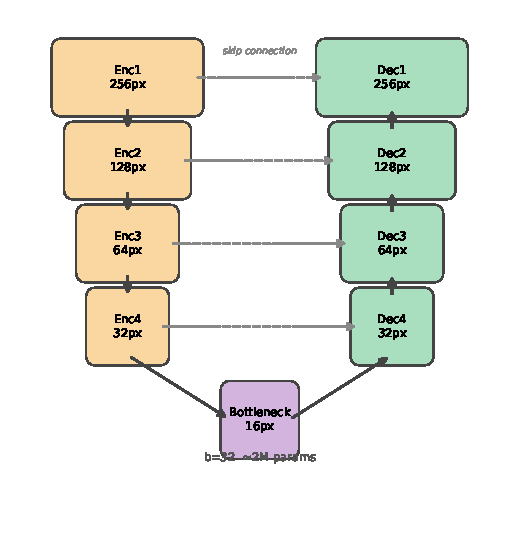
\includegraphics[width=\linewidth]{arch_unet}\\[3pt]
  \small\textbf{(c) U-Net}\\[1pt]
  \small Identical encoder/decoder plus lateral skip connections (dashed)
  that concatenate encoder feature maps at each decoder stage
  ($b{=}32$, ${\approx}2$M params).
\end{minipage}
\end{center}
\caption{The three architectures evaluated in this work. All accept a
2-channel floorplan+power input and produce a 1-channel thermal heatmap.
Encoder blocks (orange) use MaxPool2d for downsampling; decoder blocks
(green) use PixelShuffleUp for upsampling. The key structural difference
is the presence (U-Net) or absence (EncoderDecoder) of skip connections.}
\label{fig:arch}
\end{figure*}

\subsection{Baseline Architectures}

We compare two architectural baselines against U-Net to isolate the contributions
of spatial hierarchy and skip connections. Both baselines use $b {=} 64$ base
channels. The physics loss sweep ($\lambda_\text{phys} \in \{0,\,0.01,\,0.1,\,1.0\}$)
is applied to all three architectures independently, giving 12 trained models total.

\textbf{PlainCNN} ($b {=} 64$, ${\approx}600$K parameters).
Eight DoubleConv blocks in sequence at full $256\times256$ resolution. No downsampling,
no skip connections. Dilations follow the schedule $[1,\,1,\,2,\,2,\,4,\,4,\,8,\,8]$,
doubling every two blocks. By the final block the effective receptive field covers the
full input. A $1\times1$ convolution produces the output. This tests whether spatial
hierarchy is necessary for accurate hotspot localization.

\textbf{EncoderDecoder} ($b {=} 64$, ${\approx}28$M parameters).
Same four-stage encoder as U-Net ($2 \to 64 \to 128 \to 256 \to 512$ via MaxPool2d,
then a 1024-channel bottleneck) with a symmetric PixelShuffleUp decoder. The key
difference: each decoder stage receives only the upsampled feature map, not a
concatenated encoder skip. There is no \texttt{Dropout2d} in the bottleneck. This
isolates the contribution of skip connections from the effect of the physics loss.

The $\lambda_\text{phys} {=} 0$ configuration of U-Net is the direct MSE-only ablation
baseline, not a separate architecture.

\subsection{Physics-Constrained Loss}

The steady-state temperature distribution $T$ in a chip die satisfies
the 2D heat equation:
\begin{equation}
  k\,\nabla^2 T + Q = 0,
  \label{eq:heat}
\end{equation}
where $Q$ is the power-density field (channel~2 of the input image)
and $k$ is the thermal conductivity of silicon
($k \approx 149\,\mathrm{W\,m^{-1}K^{-1}}$).
In practice we set $k {=} 1.0$ during training, since thermal labels are normalized
per chip family and the physics residual must operate in the same normalized space
as $\mathcal{L}_\text{MSE}$.
Given the model's predicted
output $\hat{T}$, we approximate the Laplacian via a fixed $3\times3$
finite-difference convolution:
\begin{equation}
  \nabla^2 \hat{T} \approx \mathbf{K} \ast \hat{T},
  \qquad
  \mathbf{K} = \begin{bmatrix}
    0 & 1 & 0 \\ 1 & -4 & 1 \\ 0 & 1 & 0
  \end{bmatrix}.
  \label{eq:laplacian}
\end{equation}
The physics residual loss penalizes deviations from Equation~\ref{eq:heat}:
\begin{equation}
  \mathcal{L}_\text{phys} =
  \bigl\| k\,(\mathbf{K} \ast \hat{T}) + Q \bigr\|_F^2.
  \label{eq:phys_loss}
\end{equation}
The kernel is registered as a non-learnable buffer; gradients flow
through $\hat{T}$ only. No simulator is invoked at training time.

The composite training objective is:
\begin{equation}
  \mathcal{L} =
  \lambda_\text{data}\,\mathcal{L}_\text{MSE}(\hat{T}, T)
  +
  \lambda_\text{phys}\,\mathcal{L}_\text{phys},
  \label{eq:total_loss}
\end{equation}
where $T$ is the HotSpot ground-truth map. We sweep
$\lambda_\text{phys} \in \{0,\,0.01,\,0.1,\,1.0\}$ with
$\lambda_\text{data} = 1.0$ fixed. Because Equation~\ref{eq:phys_loss}
depends only on the prediction and the power-density input---not on
the ground-truth label---the physics constraint remains active on
OOD samples without requiring additional labeled data.

\subsection{Training Details}

All models are trained with the Adam optimizer
($\beta_1 {=} 0.9$, $\beta_2 {=} 0.999$, $\epsilon {=} 10^{-8}$,
weight decay $10^{-4}$) and an initial learning rate of $10^{-3}$.
The learning rate follows a cosine annealing schedule (CosineAnnealingLR)
with $T_\text{max} = 250$ and a minimum rate $\eta_\text{min} = 10^{-6}$.
Every model trains for exactly 250 epochs with no early stopping, and we
keep the checkpoint with the lowest validation MSE. Each run uses batch
size 8 on a single NVIDIA A10G GPU (24\,GB VRAM) via Modal.

\textbf{Per-family label normalization.} Thermal labels span different
absolute ranges across chip families (Vortex-small, Vortex-large,
NVDLA-large) because the families differ in total power. We normalize
each label by the per-family mean and standard deviation computed on
the training split, so the model sees every family's thermal structure
at a consistent scale. The power-density input to the physics loss is
divided by the mean label standard deviation across families, which
keeps the physics residual in the same normalized space as the labels.

The training loop logs MSE and physics-loss components separately per
epoch to W\&B, which lets us analyze the loss trade-off after the fact.
The physics sweep evaluates $\lambda_\text{phys} \in \{0,\,0.01,\,0.1,\,1.0\}$
across all three architectures (12 models total).

%------------------------------------------------------------------------
\section{Experiments}

\subsection{Metrics and Hyperparameter Selection}

We evaluate all models on three complementary metrics. \textbf{RMSE}
measures pixel-wise thermal accuracy in normalized units (Kelvin after
denormalization):
\begin{equation}
  \text{RMSE} = \sqrt{\frac{1}{N}\sum_{i=1}^{N}(\hat{T}_i - T_i)^2}.
  \label{eq:rmse}
\end{equation}
\textbf{Hotspot IoU} measures whether the model correctly identifies
the top-5\% hottest pixels---the spatial regions most critical for
thermal sign-off:
\begin{equation}
  \text{Hotspot IoU} =
  \frac{|\mathcal{H}_{\hat{T}} \cap \mathcal{H}_{T}|}
       {|\mathcal{H}_{\hat{T}} \cup \mathcal{H}_{T}|},
  \label{eq:iou}
\end{equation}
where $\mathcal{H}_T$ is the set of pixels in the top-5\% of the
ground-truth distribution. \textbf{SSIM} is also reported for
structural similarity but exhibits little discrimination at this
accuracy level.

All models use Adam ($\beta_1{=}0.9$, $\beta_2{=}0.999$,
$\epsilon{=}10^{-8}$, weight decay $10^{-4}$) with an initial
learning rate of $10^{-3}$ and cosine annealing over 250 epochs.
The physics weight $\lambda_\text{phys}$ is selected by grid search
over $\{0,\,0.01,\,0.1,\,1.0\}$ on the validation set;
$\lambda{=}0.01$ minimizes validation RMSE for the U-Net and is
adopted as the physics variant. Baseline architectures use
$b{=}64$ base channels; the U-Net uses $b{=}32$ because skip
connections allow competitive accuracy with fewer than 2M parameters.

\subsection{In-Distribution Results}

Table~\ref{tab:indist} reports test-set results for all four model
variants. The architectural hierarchy is clear. PlainCNN, which
processes the full $256{\times}256$ input without spatial hierarchy,
achieves the weakest performance (RMSE~$2.42$\,K, IoU~$0.630$),
indicating that a global receptive field alone is insufficient for
hotspot localization. EncoderDecoder improves substantially
(RMSE~$1.21$\,K, IoU~$0.781$) by introducing multi-scale
representations. The U-Net with lateral skip connections improves
over the encoder-decoder by 17\% in RMSE and 4.9 pp in hotspot IoU,
demonstrating that preserving high-resolution encoder features in
the decoder is critical for spatial precision.

Adding the physics penalty at $\lambda{=}0.01$ reduces U-Net RMSE
by a further 11.2\% (1.008 $\to$ 0.895\,K) and hotspot IoU by
$+2.7$ pp ($0.819 \to 0.841$). The Laplacian regularizer thus
improves in-distribution accuracy beyond what MSE alone achieves,
consistent with a physics-grounded smoothing effect.
Figure~\ref{fig:indist} visualizes the model ranking.

\begin{table}[t]
\begin{center}
\small
\begin{tabular}{@{}lccc@{}}
\toprule
Model & RMSE (K) $\downarrow$ & SSIM $\uparrow$ & Hotspot IoU $\uparrow$ \\
\midrule
PlainCNN               & 2.420 & 0.987 & 0.630 \\
EncoderDecoder         & 1.213 & 0.999 & 0.781 \\
U-Net ($\lambda{=}0$, MSE-only) & 1.008 & 0.995 & 0.819 \\
\textbf{U-Net ($\lambda{=}0.01$)} & \textbf{0.895} & \textbf{0.996} & \textbf{0.841} \\
\bottomrule
\end{tabular}
\end{center}
\caption{In-distribution test-set results. RMSE is in Kelvin (after
denormalization). Bold marks the best configuration.}
\label{tab:indist}
\end{table}

\begin{figure}[t]
\begin{center}
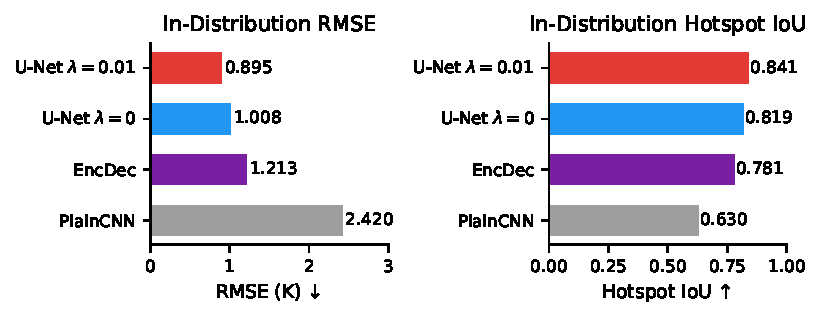
\includegraphics[width=\linewidth]{figures/indist_comparison}
\end{center}
\caption{In-distribution RMSE and hotspot IoU for all four model
variants, sorted by performance. U-Net with physics loss
($\lambda{=}0.01$) achieves the best score on both metrics.}
\label{fig:indist}
\end{figure}

\paragraph{Overfitting.}
With only 153 training instances, overfitting risk is non-trivial.
We mitigate it through three mechanisms: (1)~\texttt{Dropout2d}
($p{=}0.3$) at the bottleneck, which forces the decoder to rely on
skip-connected encoder features rather than the bottleneck alone;
(2)~weight decay ($10^{-4}$); and (3)~random horizontal and vertical
flips. The physics constraint provides additional label-independent
regularization. W\&B training curves confirm that validation MSE
tracks training MSE without divergence for the optimal U-Net variants,
while the high-$\lambda$ runs and PlainCNN show mild overfitting.

\subsection{Out-of-Distribution Generalization}

Table~\ref{tab:ood} compares the MSE-only and physics U-Net across
all eight OOD conditions; Figure~\ref{fig:ood} shows the full RMSE
curves. OOD behavior is \emph{asymmetric} across the two parameter
axes.

\textbf{Convection resistance.} At moderate shifts toward better
cooling ($r{=}0.01$\,K/W, $r{=}0.05$\,K/W), the physics-constrained
model outperforms the MSE-only baseline by 8.6\% and 10.7\%,
respectively. Both models degrade similarly at the hardest shift
($r{=}0.50$\,K/W, tenfold worse insulation), where absolute RMSE
reaches 3.9\,K for all variants---the heat-equation residual alone
cannot compensate for a shift this large.

\textbf{Die thickness.} All U-Net variants degrade severely and
nearly identically across the thickness sweep. At 300\,$\mu$m
(twice the training thickness), RMSE reaches 9.4--9.5\,K (a 9--10$\times$
increase) and hotspot IoU collapses to $\approx 0.50$, near random.
The physics penalty provides no advantage: thicker dies shift the
entire thermal range well outside the normalized training distribution,
and the Laplacian approximation cannot encode the thickness-dependent
boundary conditions.

\begin{table}[t]
\begin{center}
\small
\begin{tabular}{@{}lcc@{}}
\toprule
Condition & \makecell{U-Net\\$\lambda{=}0$} & \makecell{U-Net\\$\lambda{=}0.01$} \\
\midrule
In-dist (150\,$\mu$m, $r{=}0.1$) & 1.008 & \textbf{0.895} \\
\midrule
$r{=}0.01$\,K/W & 1.595 & \textbf{1.458} \;($-8.6\%$) \\
$r{=}0.05$\,K/W & 1.259 & \textbf{1.124} \;($-10.7\%$) \\
$r{=}0.20$\,K/W & 1.203 & \textbf{1.200} \;($\approx$0\%) \\
$r{=}0.50$\,K/W & \textbf{3.847} & 3.926 \;($+2.1\%$) \\
\midrule
75\,$\mu$m  & 6.592 & \textbf{6.428} \;($-2.5\%$) \\
100\,$\mu$m & 4.299 & \textbf{4.136} \;($-3.8\%$) \\
200\,$\mu$m & \textbf{3.137} & 3.252 \;($+3.7\%$) \\
300\,$\mu$m & \textbf{9.376} & 9.504 \;($+1.4\%$) \\
\bottomrule
\end{tabular}
\end{center}
\caption{RMSE (K) for U-Net variants across all OOD conditions.
Percentages show change relative to U-Net $\lambda{=}0$. The
physics constraint provides consistent benefit for moderate HTC
shifts but offers no advantage for die-thickness extrapolation.}
\label{tab:ood}
\end{table}

\begin{figure}[t]
\begin{center}
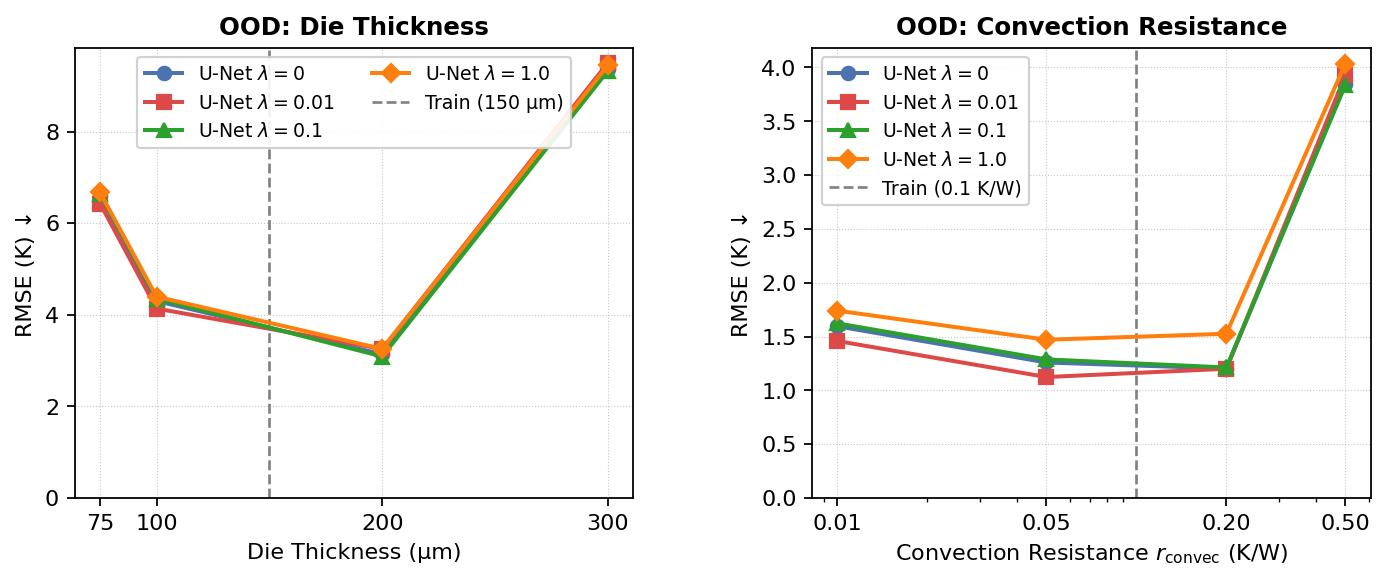
\includegraphics[width=\linewidth]{figures/ood_unet_comparison}
\end{center}
\caption{OOD RMSE for all four U-Net $\lambda$ variants. \textbf{Left:}
die-thickness sweep---all variants degrade identically; physics provides
no benefit. \textbf{Right:} convection-resistance sweep---$\lambda{=}0.01$
outperforms MSE-only at moderate shifts (0.01--0.05\,K/W) but converges
to similar error at 0.20\,K/W and 0.50\,K/W. Dashed lines mark
the training condition.}
\label{fig:ood}
\end{figure}

\subsection{Ablation Study}

Table~\ref{tab:ablation} reports the sensitivity of U-Net performance
to $\lambda_\text{phys}$. The optimal value is $\lambda{=}0.01$:
$\lambda{=}0$ leaves regularization on the table while $\lambda{=}0.1$
and $\lambda{=}1.0$ increasingly degrade RMSE ($1.036$ and $1.303$\,K,
respectively). At $\lambda{=}1.0$ the optimizer overprioritizes the
heat-equation residual at the expense of label fidelity, ultimately
yielding worse accuracy than the pure MSE-only baseline.

The final row isolates the contribution of skip connections. An
EncoderDecoder with physics loss at $\lambda{=}0.1$ achieves
competitive hotspot IoU ($0.842$) but higher RMSE ($1.190$\,K)
than U-Net~$\lambda{=}0.01$, confirming that skip connections
and physics regularization contribute orthogonally: skip connections
improve RMSE by preserving high-frequency spatial detail, while the
physics penalty improves IoU by softly enforcing thermal consistency.

\begin{table}[t]
\begin{center}
\small
\begin{tabular}{@{}lccc@{}}
\toprule
Variant & $\lambda_\text{phys}$ & RMSE (K) $\downarrow$ & Hotspot IoU $\uparrow$ \\
\midrule
U-Net                  & 0    & 1.008 & 0.819 \\
\textbf{U-Net}         & \textbf{0.01} & \textbf{0.895} & \textbf{0.841} \\
U-Net                  & 0.1  & 1.036 & 0.817 \\
U-Net                  & 1.0  & 1.303 & 0.795 \\
\midrule
EncDec (no skip conns) & 0.1  & 1.190 & 0.842 \\
\bottomrule
\end{tabular}
\end{center}
\caption{Ablation over $\lambda_\text{phys}$ and skip connections.
$\lambda{=}0.01$ minimizes RMSE; removing skip connections degrades
RMSE but maintains competitive IoU.}
\label{tab:ablation}
\end{table}

\subsection{Qualitative Results and Failure Cases}

Figure~\ref{fig:qual} shows per-family predictions from the best
model (U-Net, $\lambda{=}0.01$) on in-distribution validation samples.
Across all three chip families, the model accurately reproduces the
large-scale thermal gradient and correctly localizes the central
hotspot---the bright ring in the inferno colormap---corresponding
to the high-power compute arrays visible in the power channel.
Predicted temperatures on the GT scale align closely with ground
truth; the autoscale column confirms that the global temperature
offset is also well calibrated.

Three failure modes emerge from the OOD data.
(1)~\textbf{Thickness extrapolation}: at 75\,$\mu$m and
300\,$\mu$m, RMSE reaches 6.4--9.5\,K and hotspot IoU drops to
0.50--0.65. The thermal profile at extreme thicknesses is qualitatively
different from the 150\,$\mu$m training regime: thinner dies exhibit
steep localized gradients while thicker dies spread heat more
uniformly, both pushing the normalized prediction outside the
training distribution.
(2)~\textbf{Extreme convection shift}: at $r{=}0.50$\,K/W (tenfold
more insulating than training), all U-Net variants reach $\approx$3.9\,K
RMSE. The model has not seen the global temperature offset that
follows from poor heat dissipation, and the physics constraint
cannot encode convective boundary conditions from the Laplacian alone.
(3)~\textbf{Single-dominant-hotspot layouts}: when one block
accounts for the vast majority of total power, the MSE loss
concentrates gradient signal on that region. Fine-grained accuracy
elsewhere degrades, and hotspot IoU is sensitive to whether the
secondary hotspots---which drive real design decisions---are correctly
ranked.

\begin{figure}[H]
\begin{center}
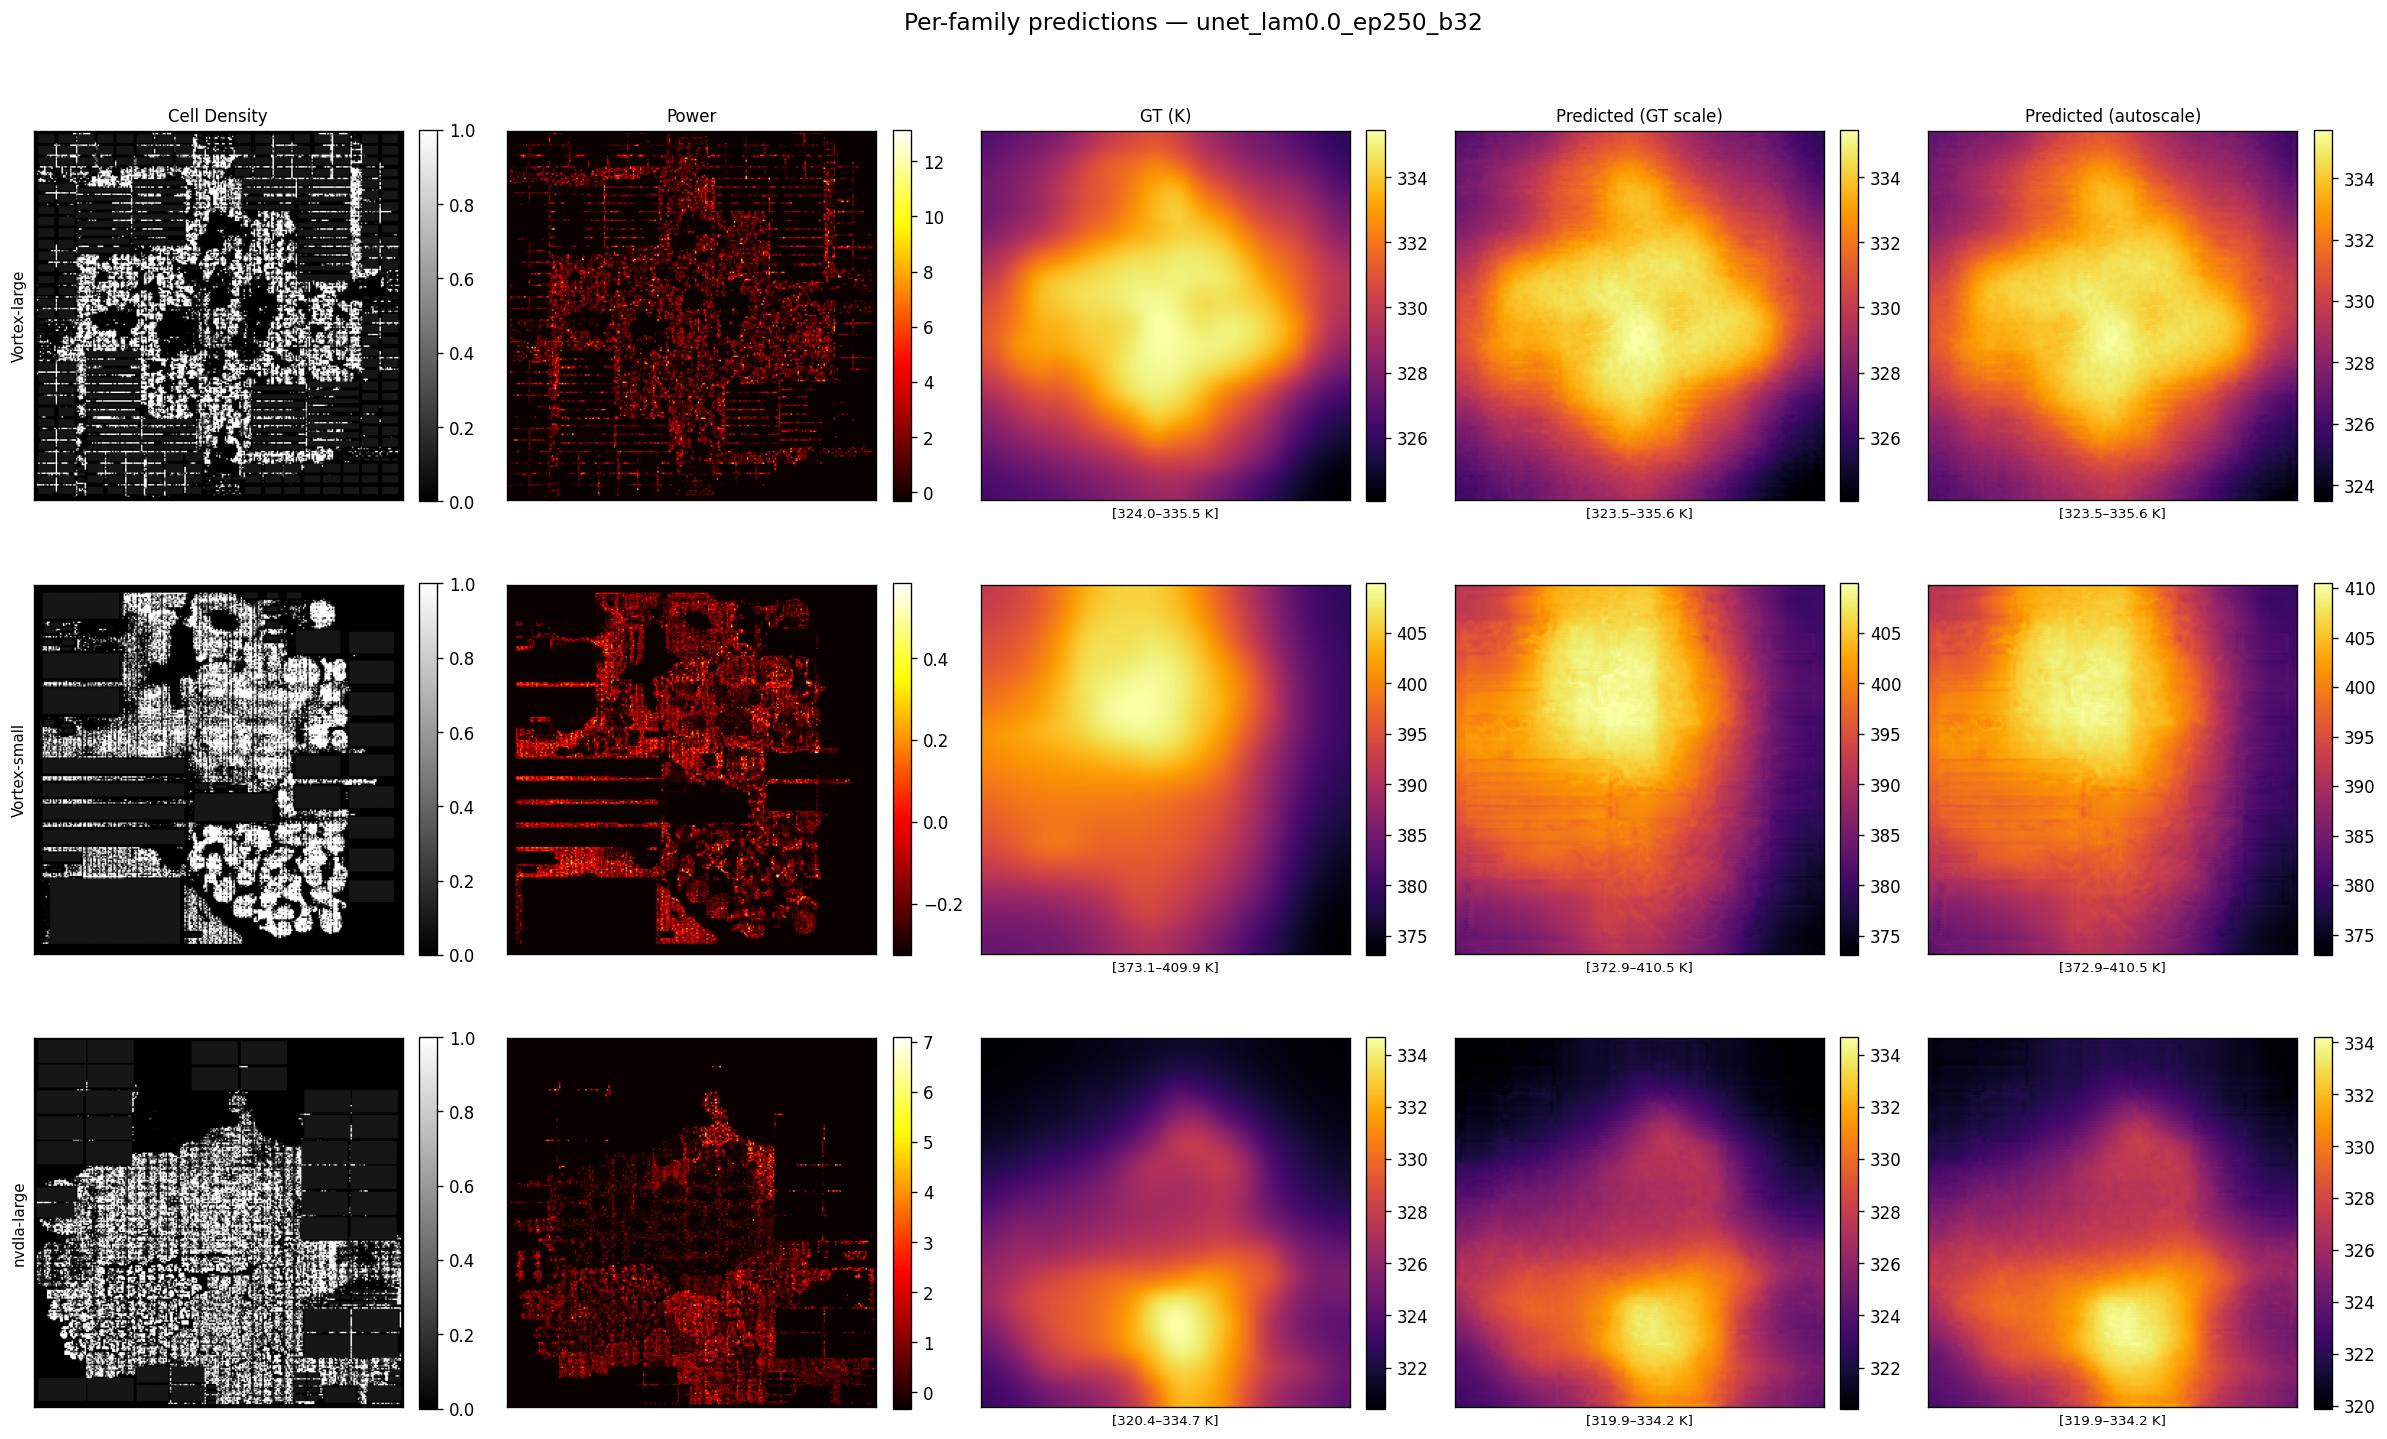
\includegraphics[width=1\linewidth]{figures/per_family_preds}
\end{center}
\caption{Per-family in-distribution predictions from U-Net
($\lambda{=}0.01$). Columns left to right: cell-density floorplan,
power-density map, HotSpot ground truth (K), model prediction on
the GT temperature scale (K), model prediction on its own autoscale.
Rows correspond to chip families (Vortex-large, Vortex-small,
NVDLA-large). The model reproduces the dominant hotspot ring and
global thermal gradient accurately across all three families.}
\label{fig:qual}
\end{figure}

%------------------------------------------------------------------------
\section{Conclusion}

We presented a physics-constrained U-Net for chip thermal map
prediction that enforces the 2D steady-state heat equation via a
differentiable Laplacian penalty computed entirely on the predicted
output. The key hypothesis is that this constraint reduces OOD
degradation on unseen die configurations by preventing the model
from predicting thermally implausible temperature fields during
extrapolation.

Our experiments confirm the in-distribution benefit of the physics
constraint: at $\lambda{=}0.01$, U-Net RMSE drops 11\% (1.008
$\to$ 0.895\,K) and hotspot IoU improves 2.7\,pp over the MSE-only
baseline. The architectural ablation establishes that skip connections
and physics regularization contribute orthogonally---skip connections
reduce RMSE by preserving high-frequency spatial detail while the
Laplacian penalty improves hotspot IoU by softly enforcing thermal
consistency. The OOD hypothesis holds \emph{partially}: the physics
constraint provides consistent 8--11\% RMSE improvement for moderate
convection-resistance shifts, but does not benefit die-thickness
generalization. All model variants degrade identically across the
thickness sweep, with RMSE reaching $9.4$--$9.5$\,K at 300\,$\mu$m.
This indicates that Laplacian regularization is a practical in-distribution
tool but that robust extrapolation across die parameters requires
stronger physics priors---such as explicit boundary condition terms---or
geometry-aware architectures.

Future directions include learning $\lambda_\text{phys}$ adaptively
during training, extending to transient thermal analysis, incorporating
boundary condition terms into the physics residual, and scaling to
3D stacked-die configurations where the volumetric heat equation
introduces additional modeling challenges.


%------------------------------------------------------------------------
\section*{Contributions}

\textbf{Fabian Molina} designed and implemented the full data pipeline:
downloading and inspecting the CircuitNet~2.0 GPU subset, writing the
\texttt{npz\_to\_hotspot.py} and \texttt{parse\_hotspot\_output.py}
conversion scripts, configuring HotSpot in grid mode with multi-block
$16{\times}16$ floorplan decomposition, and parallelizing label
generation across all 189 instances using Modal serverless workers.
Fabian authored the dataset split logic (\texttt{modal\_pipeline.py},
\texttt{scripts/make\_split.py}), per-family normalization, the
PyTorch \texttt{ThermalDataset} dataloader, and all associated unit
tests. He also wrote the Data and Methods sections of this report,
generated the architecture diagrams and data figure, and maintained
the GSD planning system and project documentation throughout.

\textbf{Ruben Carrazco} designed and implemented all three model
architectures (U-Net with pixel-shuffle upsampling, EncoderDecoder,
and PlainCNN), the full Modal training loop with W\&B logging, the
physics-constrained loss with discrete Laplacian kernel, the
CosineAnnealingLR scheduler, and the $\lambda$ sweep entrypoints.
Ruben ran all 12 model checkpoints on Modal A10G GPUs, implemented
the OOD label generation pipeline (\texttt{modal\_ood.py}) across
all eight thickness and convection-resistance conditions, wrote the
OOD evaluation script (\texttt{modal\_eval\_ood.py}), and produced
all result figures via \texttt{modal\_viz.py}. He wrote the Abstract,
Introduction, Related Work, Experiments, and Conclusion sections of
this report.

Both authors contributed to the experimental design, the physics-loss
formulation, the OOD generalization framing, and review of the final
report.

%------------------------------------------------------------------------
\section*{Acknowledgments}

We used Claude (Anthropic) as an AI assistant throughout this project.
Claude provided substantial help with the data pipeline: in particular,
we relied on it to understand how to invoke HotSpot in grid mode, how
to correctly parse the \texttt{.grid.steady} output format (which uses
a per-layer sequential-index layout rather than the column--row--temp
format described in the documentation), and how to structure the
multi-block $16{\times}16$ floorplan conversion. Claude also assisted
with LaTeX editing, figure generation scripts (\texttt{arch\_diagram.py},
\texttt{data\_figure.py}), debugging of the dataset and evaluation
code, and maintaining project planning documents. All model design
decisions, experimental methodology, result interpretation, and written
analysis are the work of the authors.

%%%%%%%%% REFERENCES
\clearpage
\bibliographystyle{ieee}
\bibliography{egbib}

\end{document}
